\documentclass[a4paper]{article}

\usepackage[utf8]{inputenc}
\usepackage[T1]{fontenc,url}
\usepackage{cite}
\usepackage{hyperref}
\usepackage{amsmath, amssymb}
\usepackage{tikz}
\usepackage{graphicx}
\usepackage{parskip}
\usepackage{lmodern}
\usepackage{algorithm}
\usepackage{algpseudocode}
\usepackage{epigraph}
\usepackage{listings}
\usepackage{float}
\usepackage{subcaption}

\begin{document}
\title{Machine learning-based approaches to denoising microseismic data}
\author{Jing Sun and Endrias Getachew Asgedom}

\maketitle
\begin{abstract}

We integrate the Convolutional Neural Network (CNN) and Strengthen-Operate-Subtract (SOS) boosting algorithm to denoise a microseismic dataset. The denoising CNN uses an autoencoder structure and learns the features of the noise in the input noisy data. The training dataset has a size of $8000\times256\times128\times1$ and the corresponding noise and signal components are obtained from a field measurement and numerical modelling, respectively. We tune the hyperparameters of the network using a grid search over the validation data. The denoising is performed by utilizing the trained model and making predictions on the test dataset. Two types of test data sets are used in this project: the first is composed of numerically modelled signal and field measured noise. The signal and noise components of the second test data are both obtained from a field measurement. For the first test dataset, the CNN-based denoising successfully removes the noise and enhances the Signal-to-Noise ratio (SNR) from $-31.146dB$ to $1.364dB$. However, the weak signals in the input data are also attenuated with the noise. For the second dataset, the network only manages to learn the features of the very strong signals in the data. Thus, it fails to preserve the weak signals. Such an aggressive denoising may be counteracted by training the CNN with additional weak signals. Finally, we enhance the results of the CNN denoising using the SOS boosting technique. Using this method with optimal hyperparameters manages to enhance the SNR from $1.364dB$ to $2.170dB$, but fails to enhance the weak signals. From visual inspection, a better enhancement of the weak signals is achieved when using hyperparameters with a poor SNR.


\noindent
\end{abstract}
\newpage

\tableofcontents

\begin{center}
    GitHub repository at \url{https://github.com/endrias34/FYS-STK4155/tree/master/Project-3}
\end{center}

\newpage

%%% MACROS
\newcommand{\half}{\frac{1}{2}}
\newcommand{\dx}{{\Delta x}}
\newcommand{\bigO}{{\mathcal{O}}}

\section{Introduction}

Denoising (or noise attenuation) is one of the long standing problems in seismic signal/image processing field. Its main aim is to attenuate the noise, the unwanted part of the data, while preserving the signal, the wanted part of the data, from a noise contaminated measurement. The most widely used denoising techniques often assume a certain kind of noise is present in the measured data, e.g., additive white Gaussian noise. Thus, to reduce such type of noise, we assume the joint probability distribution of the signal and the noise is known a prior and derive an optimal operator that minimizes the average estimation error. Recently, however, increasingly more and more learning-based denoising models, especially using a convolutional neural network (CNN), have achieved competitive or even better performance than that of the classic denoising algorithms \cite{ChenXTW18} \cite{ZhangZCM017}. On the other hand, enhancing the performance of classical denoising algorithms using the boosting method have also showed a promising success \cite{RomanoE15}. Such boosting methods treat the denoising algorithm as a $\textit{black-box}$ and adaptively build a “strong” denoising model from several “weak” ones. Nevertheless, the existing boosting algorithms still have performance gaps compared with the learning-based models \cite{ChenXTW18}. Thus, in this project, we combine the boosting algorithm named Strengthen-Operate-Subtract (SOS) \cite{RomanoE15} with that of deep CNN denoising algorithm in order to attenuate the noise and improve the Signal-to-Noise ratio (SNR) of a measured microseismic data.

This report is organized as follows: In the theory section we provide a brief introduction to the problem formulation aspect of denoising a microseismic data, then we introduce the building blocks of the CNN and SOS boosting-based denoising techniques. In the method section we present the dataset and some of the ingredients necessary for performing a machine learning-based denoising. The result and discussion sections present the main findings in this project and provide a qualitative analysis of the data. Finally, we make a concluding remark.

\section{Theory}
In this section, a brief description of the denoising problem in microseismic data analysis is given, then followed by an introduction to the theory of CNNs. In the last subsection, the basic concept of Boosting will be discussed. 

\subsection{Microseismic denoising}

Microseismic monitoring is a passive observation method where we measure the response of very small-scale earthquakes that occur as a result of human activities or industrial processes such as mining, hydraulic fracturing, enhanced oil recovery, geothermal operations or underground gas storage. These micro-earthquakes are too small to be felt on the surface by humans, but they can be detected by sensitive equipment such as geophone. 

The measurement of a microseismic monitoring event are known as microseismic data. Microseismic data are notorious for being infested with unwanted seismic and non-seismic recordings (i.e. noise). To denoise such a dataset, we consider the measured data $\mathbf{Y}\in \mathbb{R}^{N\times M}$ are obtained by combining a clean signal $\mathbf{X}\in \mathbb{R}^{N\times M}$ and a measurement noise $\mathbf{V}\in \mathbb{R}^{N\times M}$ through the following relation
\begin{equation}
\mathbf{Y} = \mathbf{X} + \mathbf{V}.
\label{eqn1}
\end{equation}
A solution to Equation \ref{eqn1} is obtained when we estimate, or separate, the unknown clean signal from the measured noise contaminated data. In this project, we estimate the clean signal using a CNN.

\subsection{Convolutional neural networks}

CNNs are a popular group of neural networks (NNs). All NNs containing one or more convolutional layers can be classified as CNNs. The complete NN can be thought of as a complicated nonlinear transformation of the input into an output that depends on the learnable weights and biases of all the neurons in the input layer, the hidden layers, and the output layer \cite{Pankaj}. A CNN is a translationally invariant NN that respects locality of the input data \cite{Pankaj}. The CNN architecture is capable of considering the local and global characteristics of the input data. Initially, CNNs have been designed to process natural image data efficiently, and for this, they were developed with properties such as local connectivity, spatial invariance, and hierarchical features \cite{MLbrain}.

\subsubsection{Convolutional layer}

The convolutional layer is the most important and essential component of a CNN. Neurons in the first convolutional layer are not connected to every single pixel in the input image, but only to pixels in their receptive fields. In turn, each neuron in the second convolutional layer is connected only to neurons located within a small rectangle in the first layer. This architecture allows the network to concentrate on the low-level features in the first hidden layer, then assemble them into higher-level features in the next hidden layer, and so on \cite{Hands-On}. 

As suggested by the name, a convolutional layer should traditionally apply a convolution operation on the input based on a bank of filter kernels (also called convolution matrix or mask) to create feature maps. All the filters of each convolutional layer have the same size. These filters are normally square matrices consisting of decimal values with a chosen size (i.e., 3$\times$3). The convolution operation is the key step that allows CNNs to be spatial invariant. The convolution operation requires flipping of the kernel and placing the kernel over the right bottom section of the image. Then, it performs a dot product between the filter parameters and the matching grid of the input. Next, the convolution operation slides the filter from right to left and bottom to top across the input.  

Consider a training data set $\left\{T_{i}, \Tilde{T}_{i}\right\}_{i=1}^{M}$  where $T$ and $\Tilde{T}$ defines the clean signals (ground truth) and noise contaminated data, respectively. We construct and train a network $f_{W,b}:\Tilde{T}_{i} \to T_{i}$ which in our case is based on a feed forward architecture. Let $N_{l}$ denote the number of features and $k_{l}=1,2,...,N_{l}$ denote the $k$’th convolutional filter in layer $l=1,2,...,L$. The feature mapping from one arbitrary layer to the next can be summarized by the expression
\begin{align}
    Z_{k_{l}}^{[l]} =
    \sum_{k_{l-1}=1}^{N_{l-1}} (W_{k_{l}}^{[l]} \ast A_{k_{l-1}}^{[l-1]})
    + B_{k_{l}}^{[l]},
    \label{conv}
\end{align}
where $W_{k_{l}}^{[l]}\in \mathbb{R}^{f_{l-1} \times f_{l-1}}$ contains the weights and $B_{k_{l}}^{[l]}$ is a matrix of same size as $Z_{k_{l}}^{[l]}$ containing the biases. The notation $\ast$ denotes the convolutional operator. 

An interesting thing to know is that with decades of development, the so-called "convolution operation" of a convolutional layer has been changed to start from the left upper of the image without flipping of the kernel. The operation will slide the kernel from left to right and top to bottom across the input \cite{MLbrain}. Even in many articles the term "convolution operation" is still kept, this operation is actually a cross-correlation operation in a mathematical standard. Most present implementations including $\mathbf{TensorFlow}$ \cite{Tensorflow}, $\mathbf{Keras}$ \cite{Keras} and $\mathbf{Pytorch}$ \cite{pytorch} replace above described convolution with the alternative cross-correlation operation. In practice, these two operations can be regarded as almost equivalent if training a CNN with filter weights being initialized using the same random procedure. Thus, training the network based on a convolutional implementation will end up with the flipped version of filter kernels as compared to alternative training based on a cross-correlation implementation. 

\subsubsection{Activation function}

In equation \ref{conv}, $A_{k_{l-1}}^{[l-1]}$ represents one of the activations from the previous layer. The activation in machine learning is defined by a non-linear transformation on all $k_{l}=1,2,...,N_{l}$ mappings of the feature maps, and defines the output from layer $l-1$ to layer $l$. The activation of layer $l$ can be represented by the general expression
\begin{align}
    A_{k_{l}}^{[l]}=\varphi^{[l]}(Z_{k_{l}}^{[l]}),
    \label{activation}
\end{align}
where $\varphi^{[l]}$ is the non-linear function. A commonly used activation function $\textit{tanh}$ is defined as
\begin{align}
    \varphi^{[l]} 
    =\frac {e^{x}-e^{-x}} {e^{x}+e^{-x}},
\end{align}
and is shown in Figure \ref{tanh}. The readers who are interested in some other popular activation functions including Sigmoid, SoftMax, ReLU and LeakyReLU can find a detailed description in \cite{project2}.

\begin{figure}[H]
  \centering
  \includegraphics[width=7cm]{Project3/tanh.png}
  \caption{The $\textit{tanh}$ activation function.}
    \label{tanh}
\end{figure}

\subsubsection{Loss function}

Loss function is a key part of the network that estimates how well the model is performing. Each time a batch (a group of training samples) is passed through the network, the loss is calculated and the parameters are updated accordingly. If the loss function is sub-optimal, the model might break down, fluctuate or take more time than needed before it converges. 

For the predicted ‘noise-free’ output of the network expressed as
\begin{align}
    \hat{T}=
    \varphi\left[\sum_{k_{L-1}=1}^{N_{L-1}} (W_{k_{L}}^{[L]} \ast A_{k_{L-1}}^{[L-1]})
    + B_{k_{L}}^{[L]} \right],
\end{align}

the mean squared error (MSE) loss function can be given by
\begin{align}
    L_{2}(W,B)=\frac{1}{2}\left \| T-\hat{T} \right\|_{2}^{2},
    \label{loss}
\end{align}
where $T$ is the ground truth.

\subsubsection{Optimizer}

The optimizer is an important building block in a NN. It is used alongside back-propagation and changes the weights and biases based on the gradient of the loss function. In essence, an optimizer has two tasks: finding the direction in which to move the weights and biases and the distance in which to move them \cite{Mitchell1997}. There are multiple different optimizers, but most have one thing in common: they are based on gradient descent. In order to find the weights and biases that minimize equation \ref{loss}, we train the network using a first-order gradient method for stochastic optimization, known as Root Mean Square propagation or RMSprop \cite{rmsprop}. The readers who are interested in the theory of back-propagation can find a detailed description in \cite{project2}.

\subsubsection{Pooling layer}

Pooling is a process of decimating the information in an image from a fine to coarse scale. Pooling layers can be classified into different categories including: max, average, and min pooling as shown in Figure \ref{pooling}. We assume the pooling has a filter size of 2$\times$2. For each region, the layer does a specific operation based on the type of pooling. The pooling types will map 4 values to one output value where: max pooling sets the output value to be the largest of the 4 values, min pooling sets the output value to be the smallest of the 4 values and average pooling computes the average of the 4 values. This process can be viewed in Figure \ref{pooling} where different regions are color coded to ease the understanding. The output of a 2$\times$2 pooling with stride 2 is a downsampling by a factor of 2 in each direction.

Pooling is much used in machine learning, and the most common type is max pooling. It is a way for the network to extract the sharpest features of an image, thus the subsequent layers after a max pooling layer will have an image consisting mainly of important features and less abundant information. Reducing the size of the input volume is also a way to increase computational speed. 

\begin{figure}[H]
  \centering
  \includegraphics[width=9.5cm]{Project3/pooling.png}
  \caption{A sketch of different types of pooling.}
    \label{pooling}
\end{figure}

\subsubsection{Upsampling}

The algorithms for upsampling include nearest neighbor and transposed convolution. The upsampling2D layer in i.e., $\mathbf{TensorFlow}$ \cite{Tensorflow} adopts the former algorithm which repeats the rows and columns of the input image to achieve the purpose of upscaling. This algorithm is often used in combination with the following convolutional layer in CNNs (i.e., autoencoders or U-Nets). Differently, the transposed convolutional layer (i.e., Conv2DTranspose in $\mathbf{TensorFlow}$ \cite{Tensorflow}) operates in a similar manner to convolutional layer, but instead of scaling an image down, the image is scaled up. The transposed convolution multiplies a value in the input with the filter values and copies it to multiple pixels as shown in Figure \ref{sampling}. The output from such layer will be weighted copies of the filter, weighted by the input. If upsampling by a factor of 2, the filter will move 2 pixels in the output for every corresponding pixel in the input.

\begin{figure}[H]
  \centering
  \includegraphics[width=9cm]{Project3/upsampling.png}
  \caption{A plot showing the process of transposed convolutional layer with a factor of 2.}
    \label{sampling}
\end{figure}

\subsection{SOS boosting}
Boosting is a widely used ensemble algorithm that improves the performance of diverse tasks by cascading several steerable sub-models \cite{ChenXTW18} \cite{Pankaj}. Several boosting-based algorithms have been used for improving the performance of image denoising algorithms \cite{ChenXTW18} \cite{RomanoE15}.  Generally, the principles of using boosting algorithm to enhance the performance of denoising algorithms can be grouped into three: (i) methods that denoise the residual, (ii) methods that enhance the denoised signal, and (iii) methods that strengthen the SNR. We use the latter approach to enhance the denoising performance of the CNN-based method. Consequently, the final denoising result inherits both the advantages of CNN and boosting. 

In this project we use the SOS boosting algorithm that treats the denoising method as a $\textit{black-box}$ and has the ability to push it forward to improve its performance. Given an initial estimation of the denoised data, the SOS algorithm improves the denoising result by performing the following iterative procedures \cite{RomanoE15}:
\begin{enumerate}
    \item Add the denoising result from the previous iteration to the input noise contaminated data to strengthen the signal.
    \item Perform denoising on the signal strengthened data from the above step.
    \item Subtract the previous denoised image from the restored signal-strengthened outcome. This guarantees the iterability of the SOS algorithm.
\end{enumerate}

Mathematically, the above procedure can be written in the following form:

\begin{equation}
\mathbf{\hat{X}^{n+1}} = \mathcal{G}(\mathbf{Y}+\mathbf{\hat{X}^n}) - \mathbf{\hat{X}^n},
\label{eqn2}
\end{equation}
where $\mathcal{G}$ is a certain denoising model imposed on the signal strengthened data, in our case it is the CNN-based denoising, and note that $\mathbf{\hat{X}^0}=\mathbf{0}$. 

Following the work of \cite{RomanoE15} we generalize the SOS boosting algorithm by introducing two parameters to it. The first parameter, $\rho$, controls the signal emphasis, and the second parameter, $\tau$ , guarantees faster convergence. Therefore, the parametrized SOS boosting algorithm may be given by

\begin{equation}
\mathbf{\hat{X}^{n+1}} = \tau\mathcal{G}(\mathbf{X}+\rho\mathbf{\hat{X}^n}) - (\tau\rho + \tau -1) \mathbf{\hat{X}^n} .
\label{eqn3}
\end{equation}

The optimal values of $\rho$ and $\tau$ can be determined by performing a grid search over the validation dataset with the SNR and $R^2$-score as the evaluation scores. 

\section{Method}

In this section, we first describe how the synthetic data sets are generated. Then, we introduce how we split the data into training, validation and test. Finally, we give a brief description of the evaluation metrics used in this project.

\subsection{Training data generation} 

As a passive observation method, the recording of a microseismic monitoring is continuous. During the measurement, a large amount of noise is recorded as a result of nearby constructions, vehicles, or passing by people and animals. These noise exists all the time and contaminate the microseismic signals. Since the micro-earthquakes do not happen all the time, the recorded data are often full of continuous noise and sparsely populated signals.

The ultimate goal of this project is to attenuate field acquired microseismic data in total absence of ground truth. To solve this problem, we use seismic forward modeling to simulate microseismic signals. By merging the synthetic microseismic signals and field recorded pure noise, we obtain field noise contaminated data with synthetic signals, here after called manually merged data. Even the synthetic microseismic signals still have many differences with the real field microseismic signals, the manually merged data can be used as the training and validation data because we have control over the ground truth. 

\subsection{Data splitting}

For the training process we split the manually merged data into three data sets: a training set, a validation set and a test set. The data sets are constructed by sorting the manually merged data randomly. The training, validation and test data sets consisted of 8000, 2000 and 50 manually merged samples (can be regarded as grey scale images) respectively. The size of each image is 256 $\times$ 128. While training, the network adjusts the weights and biases based on the difference between ground truth and the output of the network. The final model (in terms of weights and biases) is chosen according to the best fit on the validation data set. After the training and validation phases are complete, the performance of the network is checked by applying the model to the independent test data. 

The trained model is first applied on the test set of manually merged data, here after called Test set (a). By comparing the denoising results with the ground truth of Test set (a), we can accurately measure the denoising performance of the model. After that, we implement the trained model on the field recorded microseismic data set, here after called Test set (b). Due to the absence of ground truth of Test set (b), the evaluation of the model's performance will be only based on the processors' experience. In the future research, we will introduce a conventional denoising method of microseismic data as comparison of our machine learning-based methods.

Note that during the training and validation process, the model has never been able to see a field recorded microseismic image with real signals. The information of all the data sets used in this project are summarized in Table \ref{table:dataset}.

\begin{table}[H]
	\caption{Summary of the data sets}
	\centering
	\begin{tabular}{|c|c|c|c|c|c|}
		\hline
		             & Training set& Validation set& Test set (a) & Test set (b) \\  [0.5ex]
		\hline 
		Field noise  &  $\surd$  & $\surd$         & $\surd$     & $\surd$       \\ 
		\hline 
		Field signals&   $\times$ & $\times$       & $\times$    & $\surd$       \\ 
		\hline 
	Synthetic signals& $\surd$  & $\surd$          & $\surd$     & $\times$      \\ 
		\hline 
		Set size     & 8000     &   2000           &   50        & 20            \\ 
		\hline  
		Ground truth & $\surd$  & $\surd$          & $\surd$     & $\times$      \\ 
		\hline 
	\end{tabular} 
    \label{table:dataset}
\end{table}	

\subsection{Evaluation metrics}
The performance of the denoising methods can be measured using the R2-score and SNR. The $R^2$ score is a normalized error metric and its values vary between $0$ and $1$. $R^2$ represents the proportion of the variance in the dependent variable that is predictable from the independent variables. Mathematically, the $R^2$ score is given by
\begin{align}
    R^2 = 1 - \frac{\sum_{i=0}^{n - 1} (y_i - \hat{y}_i)^2}{\sum_{i=0}^{n - 1} (y_i - \bar{\mathbf{y}})^2}.
    \label{eq:R2}
\end{align}
where $\bar{\mathbf{y}}$ is the mean of $\mathbf{y}$. An $R^2$ score of $0$ means that the model is as accurate as the mean of the data and a negative score indicates that the mean is a better fit than the model.  The denoising performance of an algorithm is often quantitatively assessed via the SNR given by

\begin{align}
    SNR = 10log_{10}\frac{||\mathbf{X}_{true}||_2^2}{||\mathbf{X}_{true}-\mathbf{\hat{X}}||_2^2} ,
    \label{eq:SNR}
\end{align}
where $\mathbf{X}_{true}$ is the ground truth while $\mathbf{\hat{X}}$ is the denoising result.

\subsection{Implementation}

To perform CNN-based denoising and SOS boosting, we have used a fully object oriented Python codes with a standard $\mathbf{NumPy}$ and $\mathbf{Keras}$ libraries. Furthermore, to complement our implementation, we use unit tests to allow us to test the individual units of our source code and determine whether they are fit for use.  

\section{Results}
In this section we present the results of the denoising using a CNN and the corresponding enhancement of the results using SOS boosting algorithm.

\subsection{Denoising using CNN}

The CNN adapted in this study is a customized autoencoder. Autoencoder is a special type of NN that is commonly used for image processing in machine learning. They tend to be built up by convolutional layers, and have a specific encoder-decoder structure separating them from other types of network. Given an image, an autoencoder first encodes the image into a lower dimensional latent representation, then decodes the latent representation back to the original size. In order to represent the image at the latent layer and be able to reconstruct it back to the original size, the autoencoder has to learn which features in the data are important and which are not. Thus, the autoencoder will keep only the important features of the image and omit part of the data which contains the less important features during the contracting path. The characteristics of an autoencoder fits well with noise removal especially the type that distributes randomly. Therefore, we designed a customized autoencoder for the noise attenuation of the microseismic data. 

The architecture of our network is shown in Table \ref{AE}. The encoding and decoding functions of the autoencoder are realized by using max pooling and upsampling, respectively. Max pooling is used three times in total. The horizontal and vertical size of the image will be half of the original after each use. The number of kernels in the convolutional layer doubles as the image is compressed. Correspondingly, upsampling is also applied three times to upscale the image to its original size. The number of kernels in the convolutional layer halved as the image is decompressed. 

\begin{table} [H]
    \caption{Architecture of the customized autoencoder}

    \centering
    \begin{tabular}{p{4cm}p{4.5cm}p{1.8cm}}
        \hline
        Layer (type)       & Output Shape         & Number of Parameters \\
        \hline
        Input layer        & (None, 256, 128,   1)  & 0   \\   
        Conv $2D\_1$        & (None, 256, 128,  32) & 320 \\    
        Max Pooling $2D\_1$ & (None, 128,  64,  32)  & 0   \\ 
        Conv $2D\_2$        & (None, 128,  64,  64)  & 18496 \\   
        Max Pooling $2D\_2$ & (None,  64,  32,  64)   & 0   \\
        Conv $2D\_3$        & (None,  64,  32, 128)  & 73856\\
        Max Pooling $2D\_3$ & (None,  32,  16, 128)  & 0   \\
        Conv $2D\_4$        & (None,  32,  16, 256)  & 295168 \\  
        Up Sampling $2D\_1$ & (None,  64,  32, 256)  & 0   \\
        Conv $2D\_5$       & (None,  64,  32, 128)  & 295040\\  
        Up Sampling $2D\_2$ & (None, 128,  64, 128) & 0   \\
        Conv $2D\_6$        & (None, 128,  64,  64)  & 73792 \\ 
        Up Sampling $2D\_3$ & (None, 256, 128,  64) & 0   \\
        Conv $2D\_7$        & (None, 256, 128,  32) & 18464\\
        Output layer       & (None, 256, 128,   1)  & 289 \\
        \hline       
    \end{tabular}
    
    \centering
    \begin{tabular}{p{11.1cm}}
        \hline
        Total parameters: 775,425\\
        Trainable parameters: 775,425\\
        Non-trainable parameters: 0\\
        Filter sizes: 3$\times$3\\
        Activation function: TanH\\
        Batch size: 2\\
        Epochs: 40\\
        Loss function: MSE\\
        Optimizer: RMSprop\\
        \hline       
    \end{tabular}
    \label{AE}
\end{table} 

The proposed autoencoder has seven convolutional layers in total. The size of the filters adopted in the convolutional layers is 3$\times$3. Followed each convolutional layer the $\textit{tanh}$ activation function is applied. The loss function used in this study is MSE. The optimizer used in this study is RMSprop. To avoid the problem of overfitting, L2-norm regularization method is applied here. A grid search is used to find the optimal values of the learning rate $\eta$ and the regularization hyperparameter $\lambda$. When applying the grid search, we set the number of epochs to 40, the mini-batch size to 2. The result of the grid search is shown in Figure \ref{R2Score}. We select the optimal values for the learning rate and the regularization hyperparameter which provide the best prediction on the validation data set. In this case, we obtain an R$^2$-score of 0.897 when $\eta = 0.00025$ and $\lambda = {10}^{-6}$.

After optimizing the two hyperparameters we implement the selected trained model on the two test data sets: one is the manually merged data set, the other is acquired from the field microseismic monitoring. The denoising results are shown in Figures \ref{boosta1} and \ref{boostb1}. The CNN-based denoising on the manually merged data set improved the SNR of the noisy dataset from $-31.146$ dB to $1.364$ dB. For the field microseismic data, though we can not compute the SNR due to lack of a ground truth dataset, we can see in Figure \ref{boostb1} that the noise is highly attenuated and the strong signals in the data are preserved.

\begin{figure}[H]
  \centering
  \includegraphics[width=8.5cm]{Project3/R2Score_tanh_mse_RMSprop_l2_Input_valid.png}
  \caption{The validation R2-score for a grid search of the learning rate $\eta$ and the regularization parameter $\lambda$.}
    \label{R2Score}
\end{figure}

 

\subsection{SOS Boosting}
To improve the performance of the CNN-based denoising presented in the previous section, we use here the SOS boosting algorithm. This boosting technique has two parameters that we searched for their optimal values using a grid search over the validation dataset. Thus, these grid search using the SNR and $R^2$-score as evaluation metrics is shown in Figure \ref{boost_grid}, where we can identify the optimal $\rho$ and $\tau$ parameters to be $-0.75$ and $0.1$, respectively. However, notice that the values of the SNR and $R^2$-score corresponding to the optimal $\rho$ and $\tau$ parameters are very close to the values obtained before performing SOS boosting. Thus, one can see that the SOS boosting does not provide a significant improvement in the SNR (i.e. $2.170$ dB). However, visually inspecting the quality of the denoising result reviled that if we set $\rho=1$ and $\tau=0.7$ the weak signals in the data that are hardly recovered with the CNN denoising can now be enhanced significantly after $10$ iterations of SOS boosting (cf. Figure \ref{boosta2}). Here it is pertinent to notice that, though we managed to enhance the weak signal, its amplitude is more than that of the ground truth data, thus resulting in a lower values of SNR or $R^2$-score. 

So far we have applied the SOS boosting to a dataset that is manually merged. Now, we would like to see the performance of the SOS boosting on a dataset that has both the noise and signal components are from the field measurement. For such a dataset, we are interested in enhancing the weaker signals and not on the SNR, thus we manually set $\rho=1$ and $\tau=0.7$ and performed $10$ iterations of SOS boosting. Figure \ref{boostb2} shows the result of the denoising using the CNNs before and after SOS boosting. Here, we can see that the boosting method managed to extract the very weak signals from the noisy measurement and preserve their coherency in the spatial direction (i.e., channel direction).

\section{Discussion}

The denoising result employing the proposed autoencoder is in overall good. After the proper training process, the network managed to remove most of the noise, but damaged the very weak signals that are almost invisible in the noisy input data. Therefore, to improve the signal preservation, we may replace the upsampling + convolutional layers with the transposed convolutional layer. This is due to the fact that the upsampling layer does not have learnable weights while the transposed convolutional layer has the learnable filters. In addition, we can develop the forward modeling to simulate better synthetic signals which resembles the real microseismic signals.

The performance of the SOS boosting is unexpectedly poor in enhancing the SNR but managed to preserve weak signals from a highly noisy dataset. Thus, it is pertinent to notice that the original SOS boosting technique is designed to attenuate white Gaussian noise, but here we have a non-Gaussian noise that has similar morphology with that of the signal. Moreover, the SOS boosting is applied in \cite{RomanoE15} in an overlapping small patches of data. Thus, to improve the SNR of the SOS boosting when applied to a microseismic dataset one might attempt to apply the technique in an overlapping small patches of data. Another possible way of improving the performance of the SOS boosting technique is by combining different units of CNN at the different iterative stages of the boosting \cite{ChenXTW18}.

\begin{figure}[H]
  \centering
  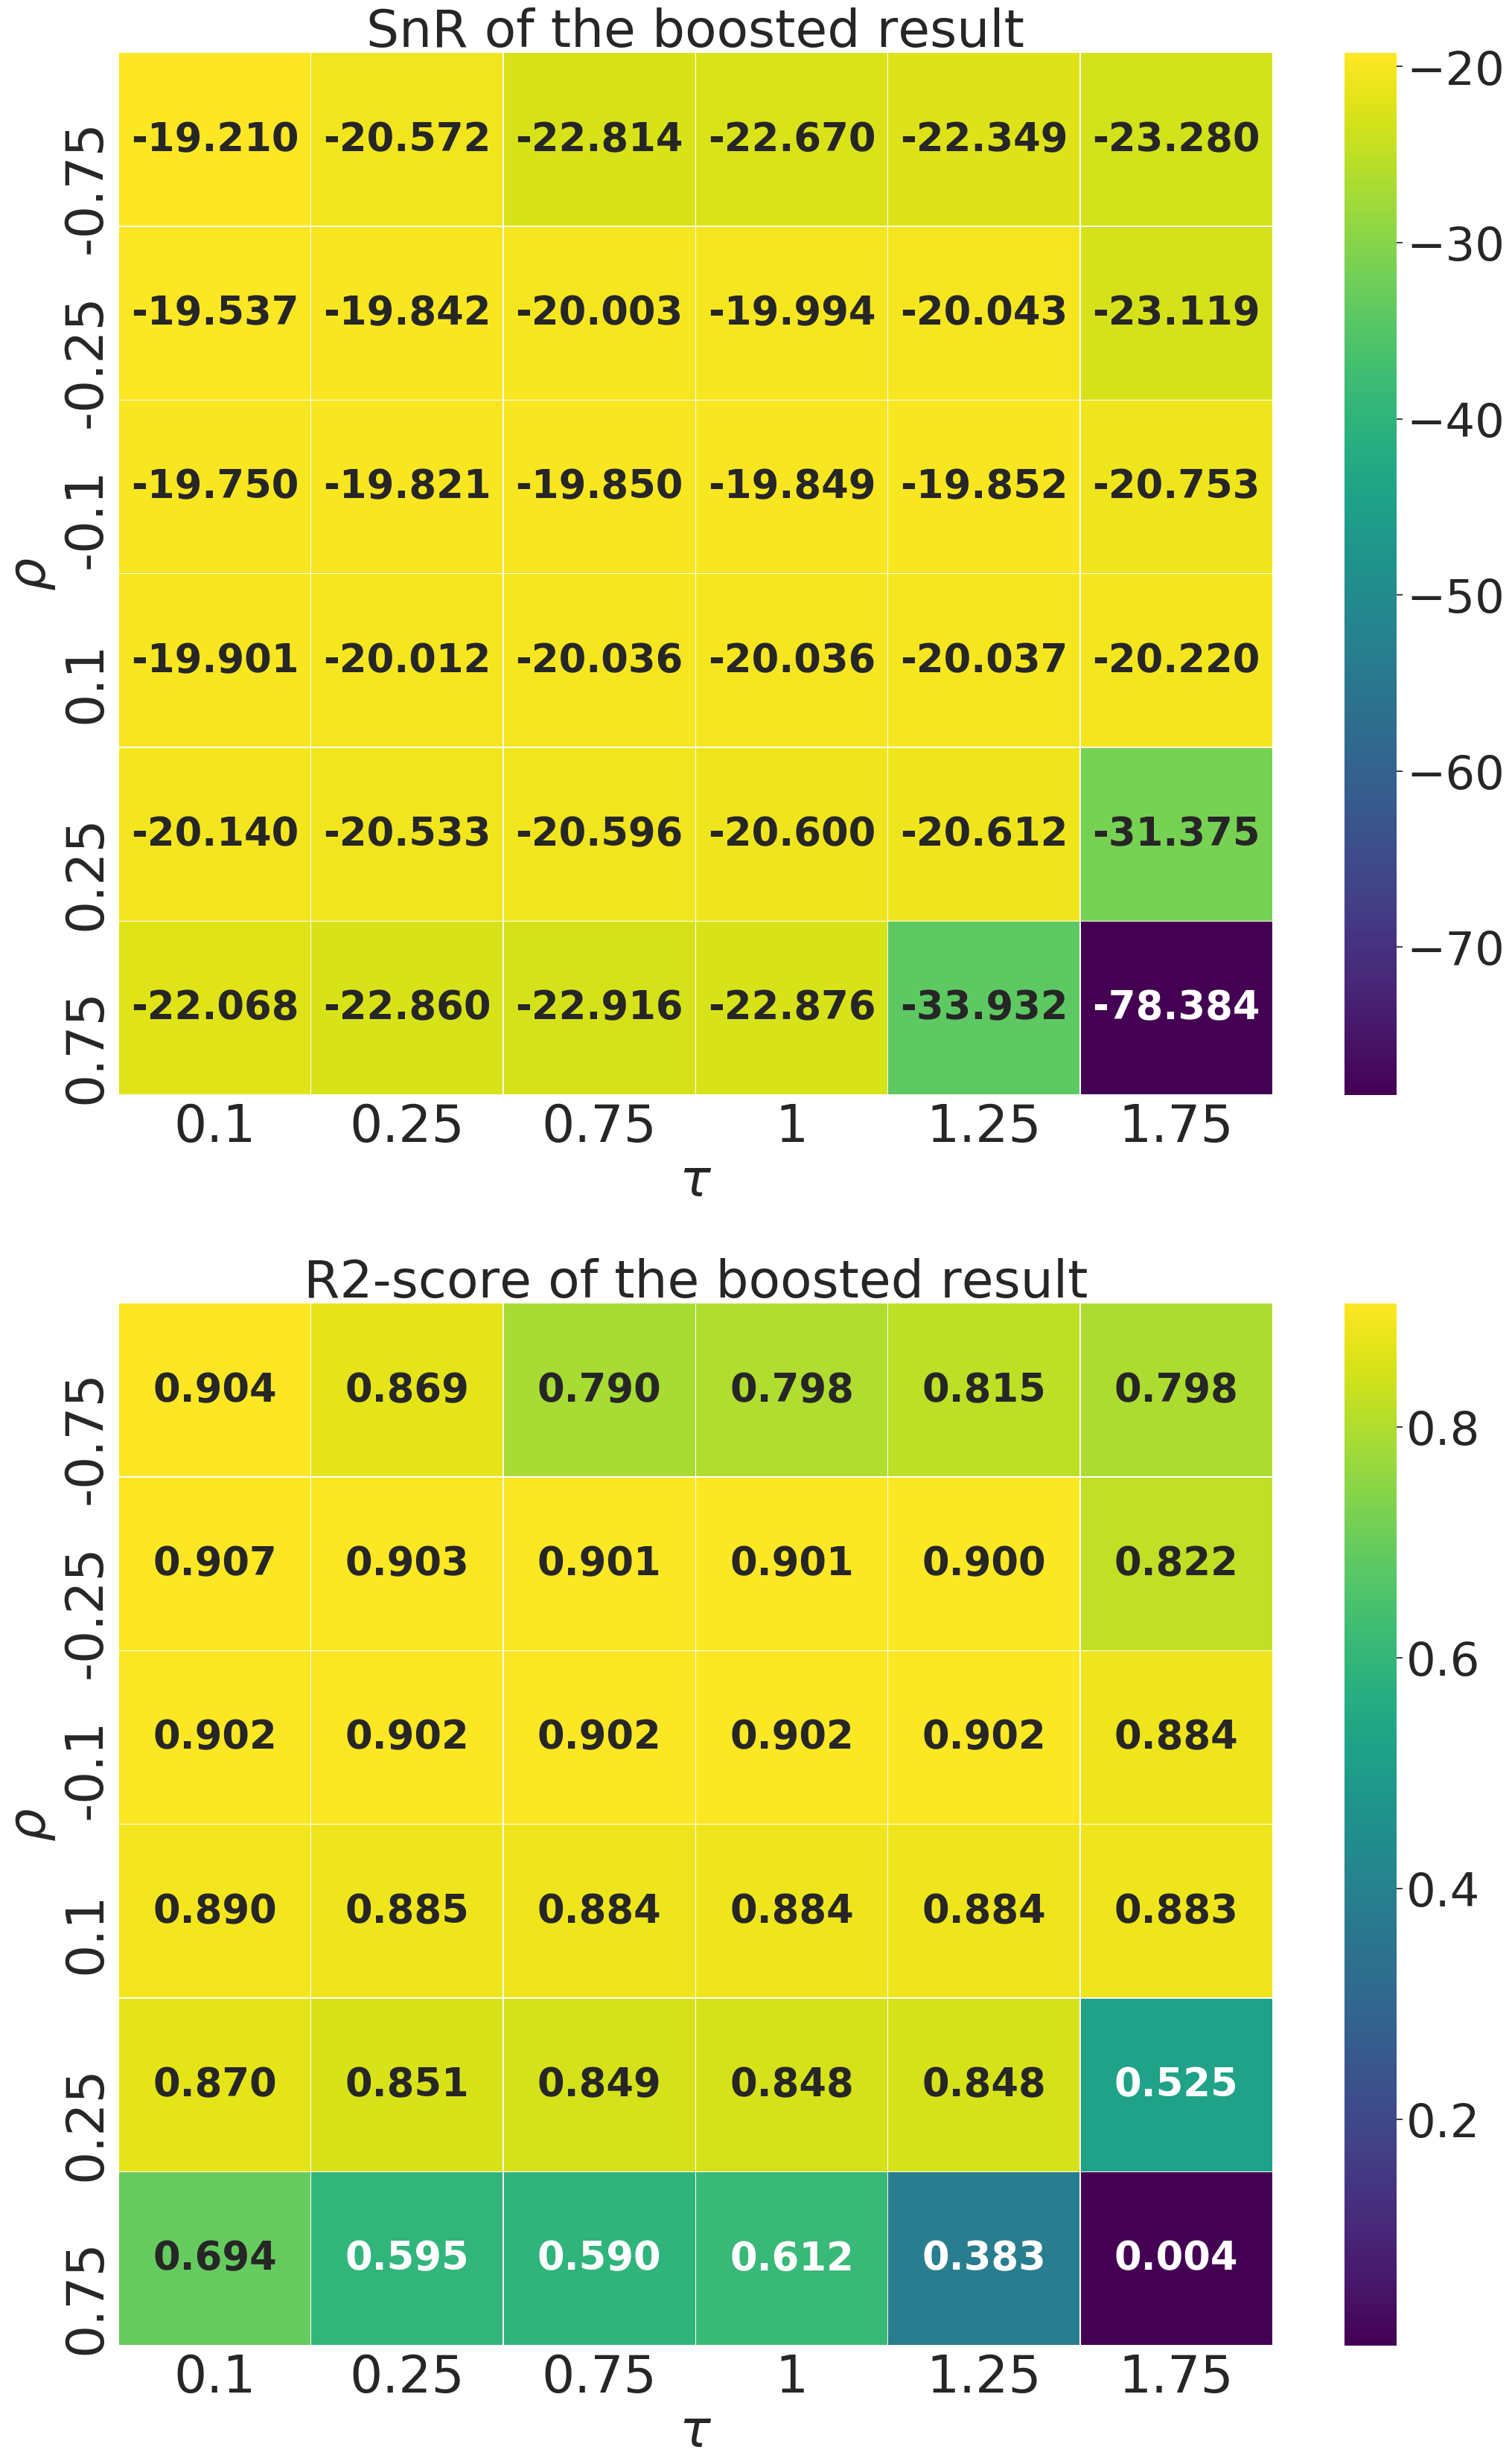
\includegraphics[width=10.5cm]{Project3/boost_grid_search.png}
  \caption{Grid search to identify the optimal values of the SOS boosting hyperparameters. Top figure shows the SNR and the bottom shows the R$^2$-score.}
    \label{boost_grid}
\end{figure}


\begin{figure}[H]
  \centering
  \includegraphics[width=8cm]{Project3/rho-0.5_tau0.1_boost_a_2.png}
  \caption{From left upper to right bottom: ground truth, manually merged noisy data, denoising result employing the proposed network and denoising result after applying SOS boosting with $\rho=-0.75$ and $\tau=0.1$.}
    \label{boosta1}
\end{figure}

\begin{figure}[H]
  \centering
  \includegraphics[width=\columnwidth]{Project3/rho-0.5_tau0.1_boost_b_19.png}
  \caption{From left to right: field recorded noisy microseismic data, denoising result employing the proposed network and denoising result after applying SOS boosting with $\rho=-0.75$ and $\tau=0.1$.}
    \label{boostb1}
\end{figure}

\begin{figure}[H]
  \centering
  \includegraphics[width=8cm]{Project3/eta0.00025_lmd1e-06_boost_a_2.png}
  \caption{From left upper to right bottom: ground truth, manually merged noisy data, denoising result employing the proposed network and denoising result after applying SOS boosting with $\rho=1$ and $\tau=0.7$.}
    \label{boosta2}
\end{figure}

\begin{figure}[H]
  \centering
  \includegraphics[width=\columnwidth]{Project3/eta0.00025_lmd1e-06_boost_b_19.png}
  \caption{From left to right: field recorded noisy microseismic data, denoising result employing the proposed network and denoising result after applying SOS boosting with $\rho=1$ and $\tau=0.7$.}
    \label{boostb2}
\end{figure}

\section{Conclusion}

We denoised a very noisy microseismic dataset using CNN and SOS boosting methods. The CNN is composed of $7$ convolutional layers, $3$ maxpooling layers, and $3$ upsampling layers. In addition, we have used $8000$ training, $2000$ validation, and $50$ test manually merged data. The optimal hyperparameters have been estimated using a grid search over the validation dataset. The CNN denoising improved the SNR from $-31.146$ dB to $1.364$ dB. In contrast, the SOS boosting after $10$ iterations with optimal parameters only achieved an SNR of $2.170$ dB. However, visually inspecting the results of SOS boosting with $\rho=1$ and $\tau=0.7$ show that the very weak signals are enhanced significantly but its corresponding SNR is lower than that of the CNN-based denoising method.

As a future work, we would like to benchmark the results of both the CNN and SOS boosting methods by comparing them with the state-of-the-art denoising method that is available in the industry. In addition, we would like to test other boosting methods, e.g., twicing \cite{Tukey77}, SAIF \cite{EsfandaraniM14}, and diffusion \cite{SzlamMC08}.


\section{Acknowledgements}
We would like to thank Professor Morten Hjorth-Jensen and the teaching assistants in the course FYS-STK-4155/3155 for the many helps we got during this project.



%\bibliographystyle{plain}
%\bibliographystyle{siam}
\bibliography{sample}
\bibliographystyle{IEEEtran}

\end{document}
